\documentclass{article}
\usepackage{polski}
\usepackage[utf8]{inputenc}
\usepackage{amsfonts}
\usepackage{amsmath}
\usepackage{latexsym}
\usepackage{longtable}
\usepackage{natbib}
\usepackage{graphicx}
\usepackage{adjustbox}
\usepackage{algorithm2e}
\usepackage{epsfig}
\usepackage{float}

\title{Sprawozdanie z listy czwartej}
\author{Karolina Bąk}
\date{Grudzień 2019}


\begin{document}
\maketitle

\section{Zadanie pierwsze}
 Celem tego zadania było zaimplementowanie funkcji obliczającej ilorazy
 różnicowe dla podanych węzłów i odpowiadających im wartości, 
 która przedstawi je w postaci wektora odpowiedniego dla 
 uogólnionego algorytmu Hornera by uzyskać postać Newtona 
 wielomianu interpolacyjnego w dalszej części listy.
\newline
 \subsection{Opis algorytmu:}

 Iloraz różnicowy \(k\)-tego rzędu można obliczyć z poniższej 
 zależności rekurencyjnej:

 $$
 \begin{aligned}
    &f[x_0] = f(x_0)\\
    &f[x_0,x_1] = \frac{f(x_1) - f(x_1)}{x_1 - x_0}\\
    &f[x_0,x_1\dots,x_k] = \frac{f[x_1,x_2\dots,x_k] - f[x_0,x_1\dots,x_{k-1}]}{x_k - x_0}\\
 \end{aligned}
 $$
\newline
 Znając węzły \(x_k\) oraz wartości funkcji \(f(x_k)\) można z pomocą wzoru 
 utworzyć macierz ilorazów różnicowych wyższych rzędów. 
 Zapisywanie całej macierzy jest nieopłacalne przez wysoką złożoność ($O(n^3)$), a do 
 poprawnej reprezentacji wystarczy jednowymiarowa tablica \(fx\). 
 Początkowymi wartościami \(fx_j\) są odpowiadające im 
 \(f[fx_j]\), obliczane ze wzoru:
 \[fx_j = \frac{fx_j - fx_{j-1}}{x_j - x_{j-i}},\] gdzie 
 \(i\) jest numerem kolumny w macierzy. Każda 
 następna wartość jest aktualizowana kolumnami w kolejności z 
 dołu do góry. Dzięki temu tablica 
 \(fx\) w każdym momencie posiada wartości ilorazów potrzebne dla następnych 
 kroków algorytmu.
 \newline
 \newline
 
\subsection{Pseudokod:}

\begin{algorithm}
    \DontPrintSemicolon
    \KwIn{Wektor $x$ długości n+1 węzłów oraz wektor $f$ zawierający wartości funkcji interpolowanej w tych węzłach} 
    \KwOut{Wektor $fx$ długości n+1 obliczonych ilorazów różnicowych}
    \;
    $ ln \gets length(f)$
    $ fx  \gets copy(f)$
    \;
    \For{$i \gets 2$ \textbf{to} $ln$} {
        \For{$j \gets ln$ \textbf{to} $i$} {
            $fx[j] = (fx[j] - fx[j - 1]) / (x[j] - x[j - i + 1])$
        }
    }
    \;
    \Return{$fx$}
\end{algorithm}

\section{Zadanie drugie}
Celem tego zadania było napisanie funkcji obliczającej 
wartość wielomianu interpolacyjnego stopnia $n$ w postaci 
Newtona $N_n(x)$ w punkcie $x = t$ za pomocą uogólnionego 
algorytmu Hornera, działającą w czasie $O(n)$.
\newline

\subsection{Opis algorytmu:}
Wielomian interpolacyjny Newtona jest zadany wzorem:
\[N_n(x) = \sum_{i=0}^k c_i \prod_{j=0}^{i-1}(x - x_j) ,\]
gdzie $c_i$ jest ilorazem różnicowym stopnia $i$, a 
$x_j$ węzłem interpolacji.
\newline
Aby obliczyć wartość tego wielomianu w danym punkcie 
można użyć uogólnionego algorytmu Hornera. Jego działanie 
można przedstawić następującymi zależnościami:
$$
\begin{aligned}
    &w_n(x) = f[x_0, x_1 \dots, x_n] \\
    &w_k(x) = w_{k+1}(x-x_k) + f[x_0, x_1 \dots, x_k] \\
    &N_n(x) = w_0(x)
\end{aligned}
$$
Jeśli ilorazy są już obliczone, to zastosowanie powyższych wzorów 
pozwala znaleźć wartość wielomianu w czasie liniowym.
\newline
\newline
\newline
\subsection{Pseudokod:}\quad
\begin{algorithm}
    \DontPrintSemicolon
    \KwIn{Wektory $x$ i $fx$ zawierające odpowiednio 
    węzły i ilorazy różnicowe długości n+1 oraz $t$ jako 
    punkt, w którym należy obliczyć wartość wielomianu}
    \KwOut{Wartość wielomianu w punkcie $nt$}
    \;
    $ln \gets length(x)$
    $nt \gets fx[ln]$
    \;
    \For{$i \gets ln-1$ \textbf{to} $1$} {
        $nt \gets fx[i] + (t - x[i]) * nt$
    }
    \;
    \Return{$nt$}
\end{algorithm}

\section{Zadanie trzecie}
Celem zadania było napisać funkcję obliczającą 
w czasie \(O(n^2)\) współczynniki postaci naturalnej 
dla podanych współczynników wielomianu interpolacyjnego 
Newtona oraz węzłów \(x_0, \dots, x_n\).

\subsection{Opis algorytmu:}
Postać naturalną wielomianu stopnia $n$ zmiennej $x$ 
można przedstawić wyrażeniem:
\[\sum_{i=0}^{n} a_ix^i\]
Aby znaleźć współczynniki wielomianu interpolacyjnego 
w postaci naturalnej należy jako punkt wyjścia obrać 
uogólniony algorytm Hornera z poprzedniego zadania. 
Współczynnik $a_n$ w szukanym wielomianie $n$-tego 
stopnia (przy najwyższej potędze x) jest równy $c_n$, z czego 
wynika, że $w_n$ z algorytmu Hornera jest także równe $a_n$. 
\newline
\newline
Posiadając początkowe warunki dla algorytmu w następnych 
krokach tworzone są wartości $a_i$ opierające się na 
współczynnikach $a_{i+1}$. Aby znaleźć zależności 
między następnymi $a_i$ algorytm przechodzi po 
wszystkich $w_i$ od $i$ równego $n$ do $0$, zmieniając 
tworzone współczynniki, tak aby dla każdego $w_i$ 
doprowadzić w danej chwili do postaci naturalnej.
\newline
\newline
\newline
\subsection{Pseudokod:}\quad
\begin{algorithm}
    \DontPrintSemicolon
    \KwIn{Wektory $x$ i $fx$ długości n+1 zawierające węzły $x_0 \dots x_n$ oraz ilorazy różnicowe}
    \KwOut{Wektor $a$ długości n+1 zawierający obliczone współczynniki postaci naturalnej}
    \;
    $ln \gets length(x)$
    $a \gets zeros(ln)$
    $a[ln] \gets fx[ln]$
    \;
    \For{$i \gets ln -1$ \textbf{to} $1$} {
        $a[i] \gets fx[i] - a[i + 1] * x[i]$
        \For{$j \gets i+1$ \textbf{to} $ln-1$} {
            $a[j] \gets a[j] - a[j + 1] * x[i]$
        }
    }
    \;
    \Return{$a$}
\end{algorithm}

\section{Zadanie czwarte}
Celem zadania było napisać funkcję, która interpoluje 
zadaną funkcję $f(x)$ w przedziale $[a,b]$ za pomocą 
wielomianu interpolacyjnego $n$-tego stopnia w postaci 
Newtona, a następnie narysuje interpolowany wielomian 
oraz interpolowaną funkcję.

\subsection{Opis algorytmu:}
Do reprezentacji graficznej, aby uzyskać dobre efekty w interpolacji użyłam
węzłów równo od siebie oddalonych w podanym przedziale. Wyznaczam je w następujący sposób:
$$
\begin{aligned}
    &x_k = a + kh  
    &k = 0, 1 \dots n\\
    &h = \frac{b-a}{n}
\end{aligned}
$$
\newline
Wielomian interpolacyjny nie był jawnie obliczany, gdyż wystarczyło 
tylko użyć funkcji z pierwszych dwóch zadań. Najpierw iteracyjnie wyznaczyłam 
wektor węzłów i wartości funkcji im odpowiadające. Z nich uzyskałam 
przy użyciu funkcji \textit{ilorazyRoznicowe} wektor ilorazów pod algorytm Hornera. 
Następnie obliczyłam wartości wielomianu dla punktów na wykresie, korzystając 
z funkcji \textit{warNewton}. 
\newline
\newline
Ostatnim krokiem algorytmu było narysowanie 
wykresów funkcji oraz interpolowanego wielomianu. Do tej części użyłam pakietu 
PyPlot (pakiet z języka Python importowany do Julii).
Liczba punktów narysowanych na wykresie jest 
dwadzieścia razy większa niż ilość węzłów użytych do wyznaczenia wielomianu 
w celach estetycznych. Nie ma to wpływu na dokładność interpolacji, gdyż 
liczba węzłów i ilorazów różnicowych nie jest zwiększana. 

\subsection{Pseudokod:}
\begin{algorithm}
    \DontPrintSemicolon
    \KwIn{Funkcja $f$, końce przedziału $a,b$ na którym będzie interpolowana funkcja, ilość węzłów $n$ }
    \KwOut{Wykres funkcji oraz wielomianu na danym przedziale}
    \;
    $maxnodes \gets n+1$
    \;
    $x[maxnodes]$
    $y[maxnodes]$
    $fx[maxnodes]$
    \;
    $plotargs[20*maxnodes]$
    $plotval[20*maxnodes]$
    $plotip[20*maxnodes]$
    \;
    $kh \gets 0$
    $h \gets (b-a)/n$
    \;
    \For{$i \gets 1$ \textbf{to} $maxnodes$}{
        $x[i] \gets a + kh$\;
        $y[i] \gets f(x[i])$\;
        $kh \gets kh + h$
    }
    $fx \gets ilorazyRoznicowe(x,y)$\;
    $kh \gets 0$
    $maxnodes \gets maxnodes*20$
    $h \gets (b-a)/(maxnodes-1)$\;
    \For{$i \gets 1$ \textbf{to} $maxnodes$}{
        $plotargs[i] \gets a + kh$\;
        $plotip[i] \gets warNewton(x,fx,plotargs[i])$\;
        $plotval[i] \gets f(plotargs[i])$\;
        $kh \gets kh + h$
    }
    $clf()$\;
    $plot(plotargs,plotval,"f(x)")$\;
    $plot(plotargs,plotip,"w(x)")$\;
    $savefig("plot.png")$
\end{algorithm}

\section{Zadanie piąte}
Celem zadania było przetestowanie funkcji z poprzedniego 
zadania $rysujNnfx(f,a,b,n)$ na następujących 
przykładach:

\begin{itemize}
    \item $e^x, [0,1], n=5,10,15$;
    \item $x^2\sin x, [-1,1], n=5,10,15$.
\end{itemize}
\quad\newline
Poniżej przedstawiam uzyskane wyniki. Jak można 
zaobserwować, już dla 5 węzłów interpolowany 
wielomian pokrywa się z funkcją.

\begin{figure}[H]
    \centering
    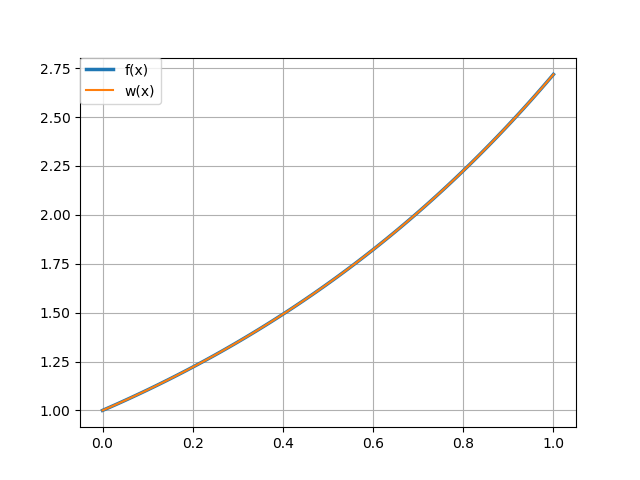
\includegraphics[width=0.65\textwidth]{plots/5a_5.png}
    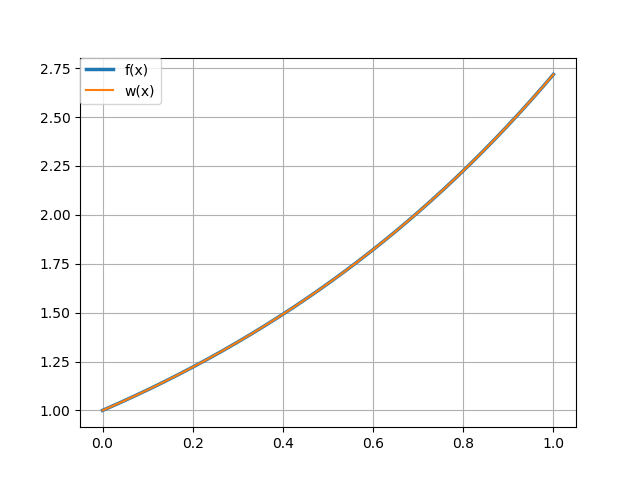
\includegraphics[width=0.65\textwidth]{plots/5a_10.png}
    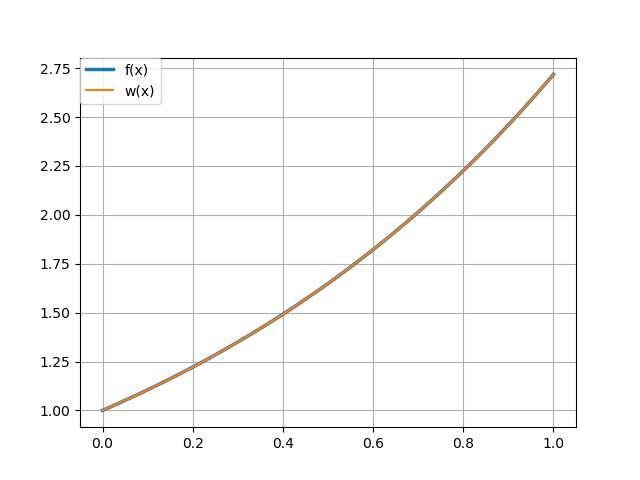
\includegraphics[width=0.65\textwidth]{plots/5a_15.png}
    \caption{Wykresy funkcji $e^x$ oraz wielomianu interpolującego na przedziale 
    $[0,1]$ dla $n=5,10,15$}
\end{figure}

\begin{figure}[H]
    \centering
    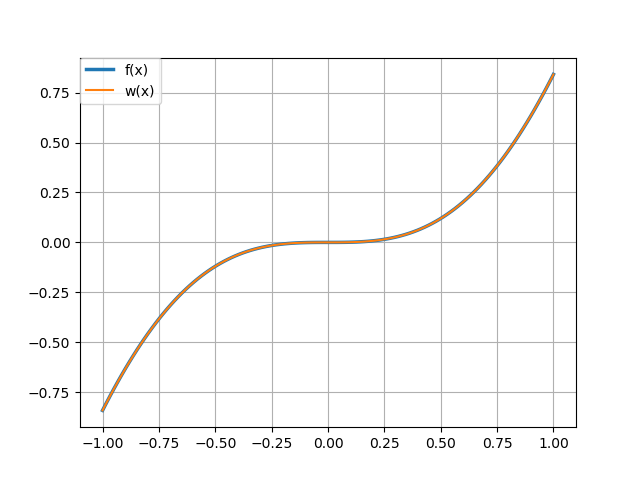
\includegraphics[width=0.65\textwidth]{plots/5b_5.png}
    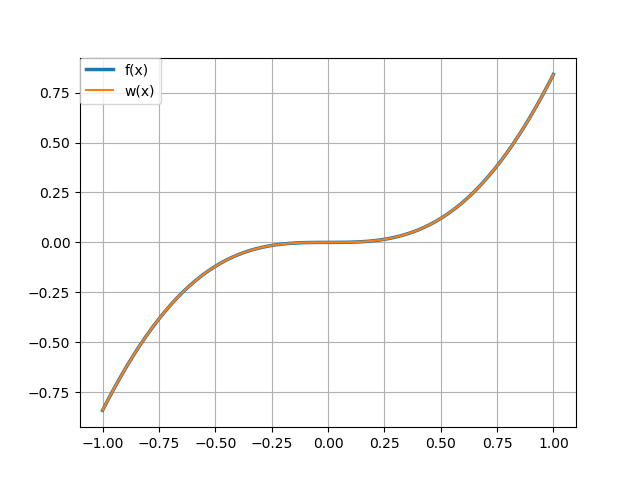
\includegraphics[width=0.65\textwidth]{plots/5b_10.png}
    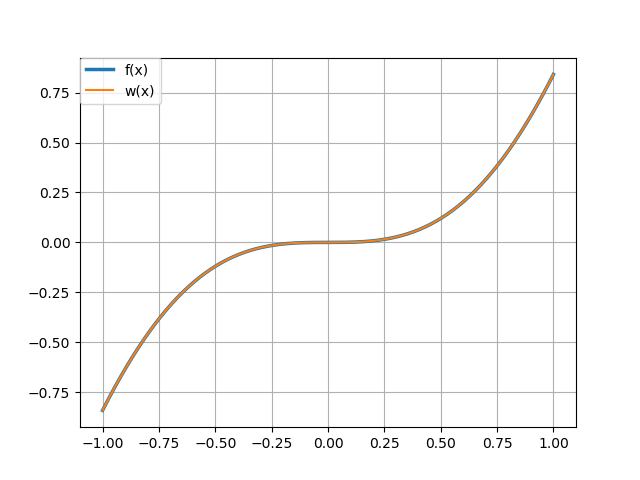
\includegraphics[width=0.65\textwidth]{plots/5b_15.png}
    \caption{Wykresy funkcji $x^2\sin x$ oraz wielomianu interpolującego na przedziale 
    $[-1,1]$ dla $n=5,10,15$}
\end{figure}

\section{Zadanie szóste}
Celem zadania było przetestowanie funkcji  
$rysujNnfx(f,a,b,n)$ na ciekawszych 
przykładach:

\begin{itemize}
    \item $|x|, [-1,1], n=5,10,15$;
    \item $\frac{1}{1+x^2}, [-5,5], n=5,10,15$.
\end{itemize}
\quad\newline
Otrzymane wykresy znajdują się 
na kolejnych stronach. Można na 
nich zauważyć, że interpolacja 
nawet dobrze zaimplementowana jest 
podatna na błędy. Widoczne jest to 
zwłaszcza przy funkcjach, które ciężko 
przedstawić w formie wielomianu - na przykład 
$|x|$. 
\newline
\newline
Aby dokładność wzrosła można 
zwiększyć ilość węzłów, jednak nie 
zawsze uzyskuje się lepszą dokładność - $|x|$ 
dla $n = 10$. Na ogół jednak, jeśli 
zwiększymy stopień wielomianu to 
dostaniemy lepszą dokładność w środku przedziału. 
Niestety na krańcach przedziału pojawiają się wtedy 
duże wahania - widoczne szczególnie w 
$\frac{1}{1+x^2}$ dla $n = 10,15$. 
Te zaburzenia są spowodowane charakterystyką 
badanych funkcji i nie można ich 
uniknąć przy węzłach równoodległych.
\newline
\newline
Z przeprowadzonych testów można 
wywnioskować, że interpolacja jest dobrym 
narzędziem do przybliżania funkcji. 
Jednak trzeba uważać przy korzystaniu 
z niej, gdyż są funkcje, które 
wymagają odpowiedniego rozstawienia 
węzłów do ich poprawnego 
przedstawienia, a jeśli nie wiemy 
jakiej funkcji się spodziewać możemy 
wysunąć błędne wnioski lub uzyskać 
błędne wyniki.

\begin{figure}[H]
    \centering
    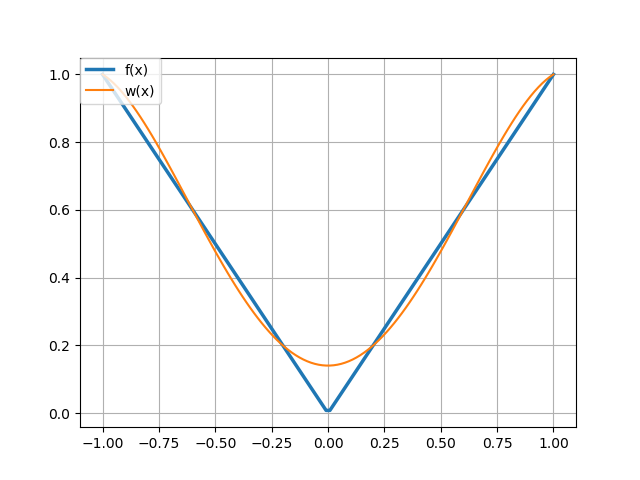
\includegraphics[width=0.65\textwidth]{plots/6a_5.png}
    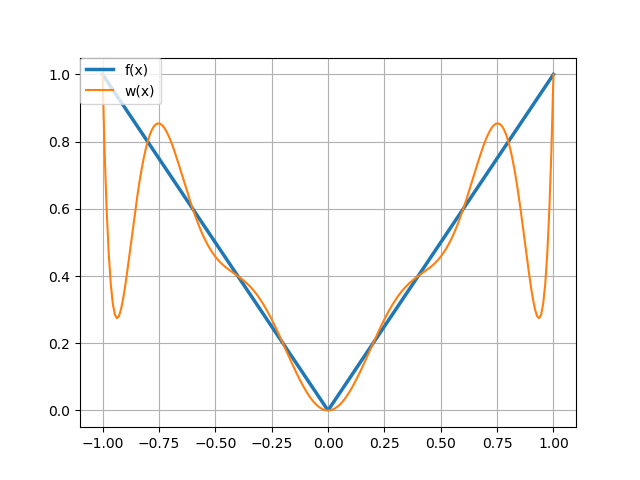
\includegraphics[width=0.65\textwidth]{plots/6a_10.png}
    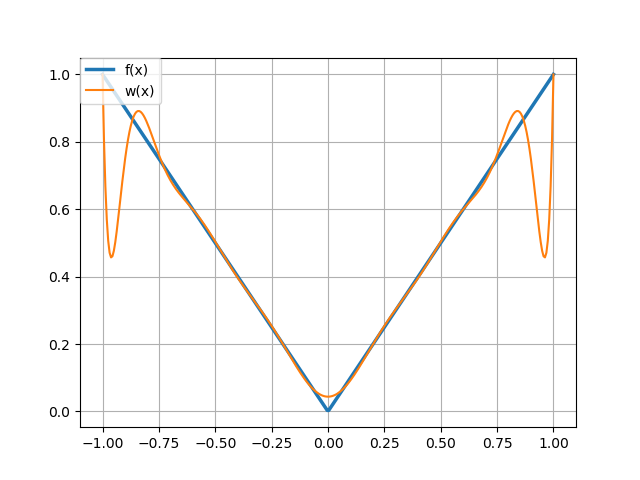
\includegraphics[width=0.65\textwidth]{plots/6a_15.png}
    \caption{Wykresy funkcji $|x|$ oraz wielomianu interpolującego na przedziale 
    $[-1,1]$ dla $n=5,10,15$}
\end{figure}

\begin{figure}[H]
    \centering
    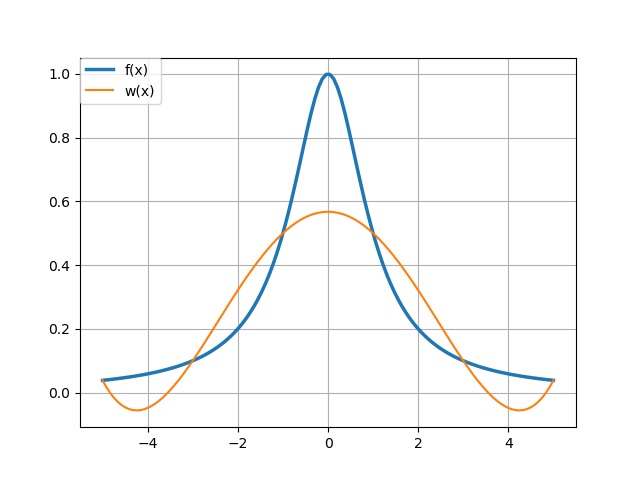
\includegraphics[width=0.65\textwidth]{plots/6b_5.png}
    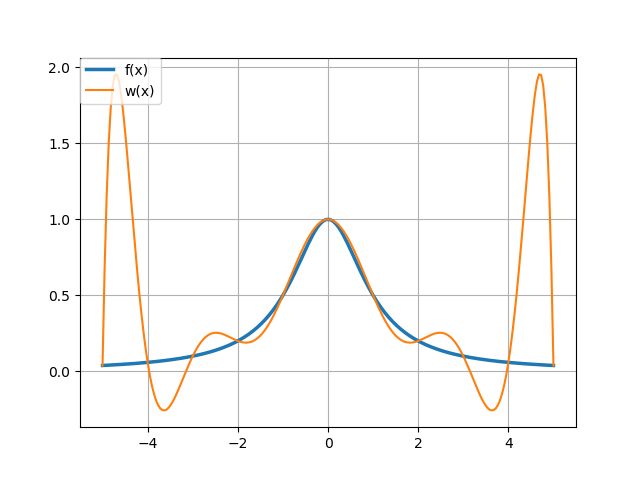
\includegraphics[width=0.65\textwidth]{plots/6b_10.png}
    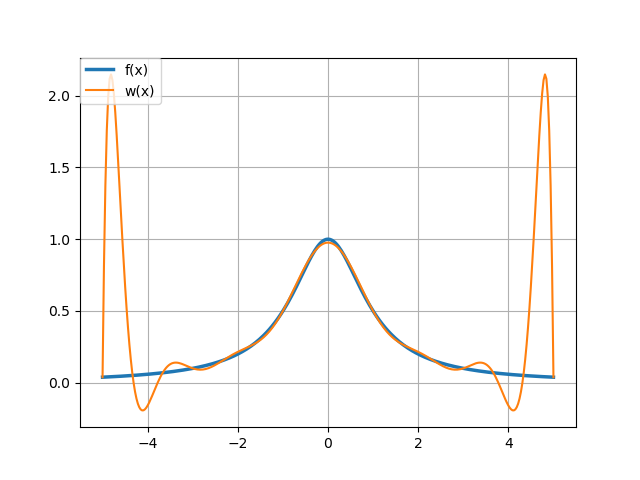
\includegraphics[width=0.65\textwidth]{plots/6b_15.png}
    \caption{Wykresy funkcji $\frac{1}{1+x^2}$ oraz wielomianu interpolującego na przedziale 
    $[-5,5]$ dla $n=5,10,15$}
\end{figure}

    
\end{document}